\documentclass[10pt,a4paper]{article}
\usepackage{tikz}
\usepackage{tkz-euclide} % loads  TikZ and tkz-base
\usetkzobj{all}
\begin{document}
\providecommand{\brak}[1]{\ensuremath{\left(#1\right)}}

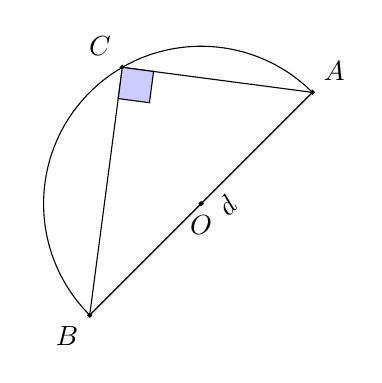
\begin{tikzpicture}
  [
    scale=2,
    >=stealth,
    point/.style = {draw, circle,  fill = black, inner sep = 0.5pt},
  ]
  \def\rad{1}
 \coordinate [point, label={below :	$O$ }] (O) at (0, 0);
    \node (A) at +(45:{\rad}) [point,label = above right:$A$ ] {};  
    \node (B) at +(225:{\rad}) [point,label = below left:$B$ ] {};      
    \node (C) at +(120:{\rad}) [point,label = above left:$C$ ] {};          
  \path
     (B)    edge  node[sloped, anchor=east, below right, text width=0.5cm] { $d$}     (A) ; 
  \draw (A) -- (C);
  \draw (B) -- (C);
\draw
    (A) arc(45:225:\rad) -- cycle;
  \tkzMarkRightAngle[fill=blue!20,size=.2](A,C,B)        
     
\end{tikzpicture}

\end{document}